\documentclass[12pt, twoside]{book}

% variable values
\input variables.tex

\ifshowframe{}
    \usepackage[a4paper,top=2.5cm,bottom=2.5cm,left=3.5cm,right=2cm,showframe]{geometry}
\else
    \usepackage[a4paper,top=2.5cm,bottom=2.5cm,left=3.5cm,right=2cm]{geometry}
\fi
\usepackage{microtype}
\usepackage[slovak,USenglish]{babel}
\usepackage[utf8]{inputenc}
\usepackage[T1]{fontenc}

\linespread{1.25} % this means 1.5 line spacing

% more package imports and custom commands
\input definitions.tex

\tikzset{every node/.style={circle, draw, fill=black}}

\begin{document}

\ifenglish{}
    \selectlanguage{USenglish}
\else
    \selectlanguage{slovak}
\fi

\frontmatter
\pagenumbering{gobble}

% COVER
\thispagestyle{empty}

{
    \sc\large

    \begin{center}
        \thesisuniversity{}\\
        \thesisfaculty{}

        \vfill

        {\LARGE\thesisname}\\
        \thesistype{}
    \end{center}

    \vfill

    \noindent
    \thesisyear{}\\
    \thesisauthor{}
}

\cleardoublepage{}

% TITLE PAGE
\frontmatter
\thispagestyle{empty}

\begin{center}
    \sc\large
    \thesisuniversity{}\\
    \thesisfaculty{}

    \vfill

    {\LARGE\thesisname}\\
    \thesistype{}
\end{center}

\vfill

\noindent
\begin{tabular}{ll}
    \ifenglish{}Study Programme:\else{}Študijný program:   \fi & \thesisprogramme{}\\
    \ifenglish{}Field of Study: \else{}Študijný odbor:     \fi & \thesisfield{}\\
    \ifenglish{}Department:     \else{}Školiace pracovisko:\fi & \thesisdepartment{}\\
    \ifenglish{}Supervisor:     \else{}Školiteľ:           \fi & \thesissupervisor{}\\
    \ifconsultant{}\ifenglish{}Consultant:\else{}Konzultant:\fi & \thesisconsultant{}\\ \fi
\end{tabular}

\vfill

\noindent
\thesislocation, \thesisyear{}\\
\thesisauthor{}

\cleardoublepage{}

% ASSIGNMENT
\newpage
\thispagestyle{empty}

\noindent
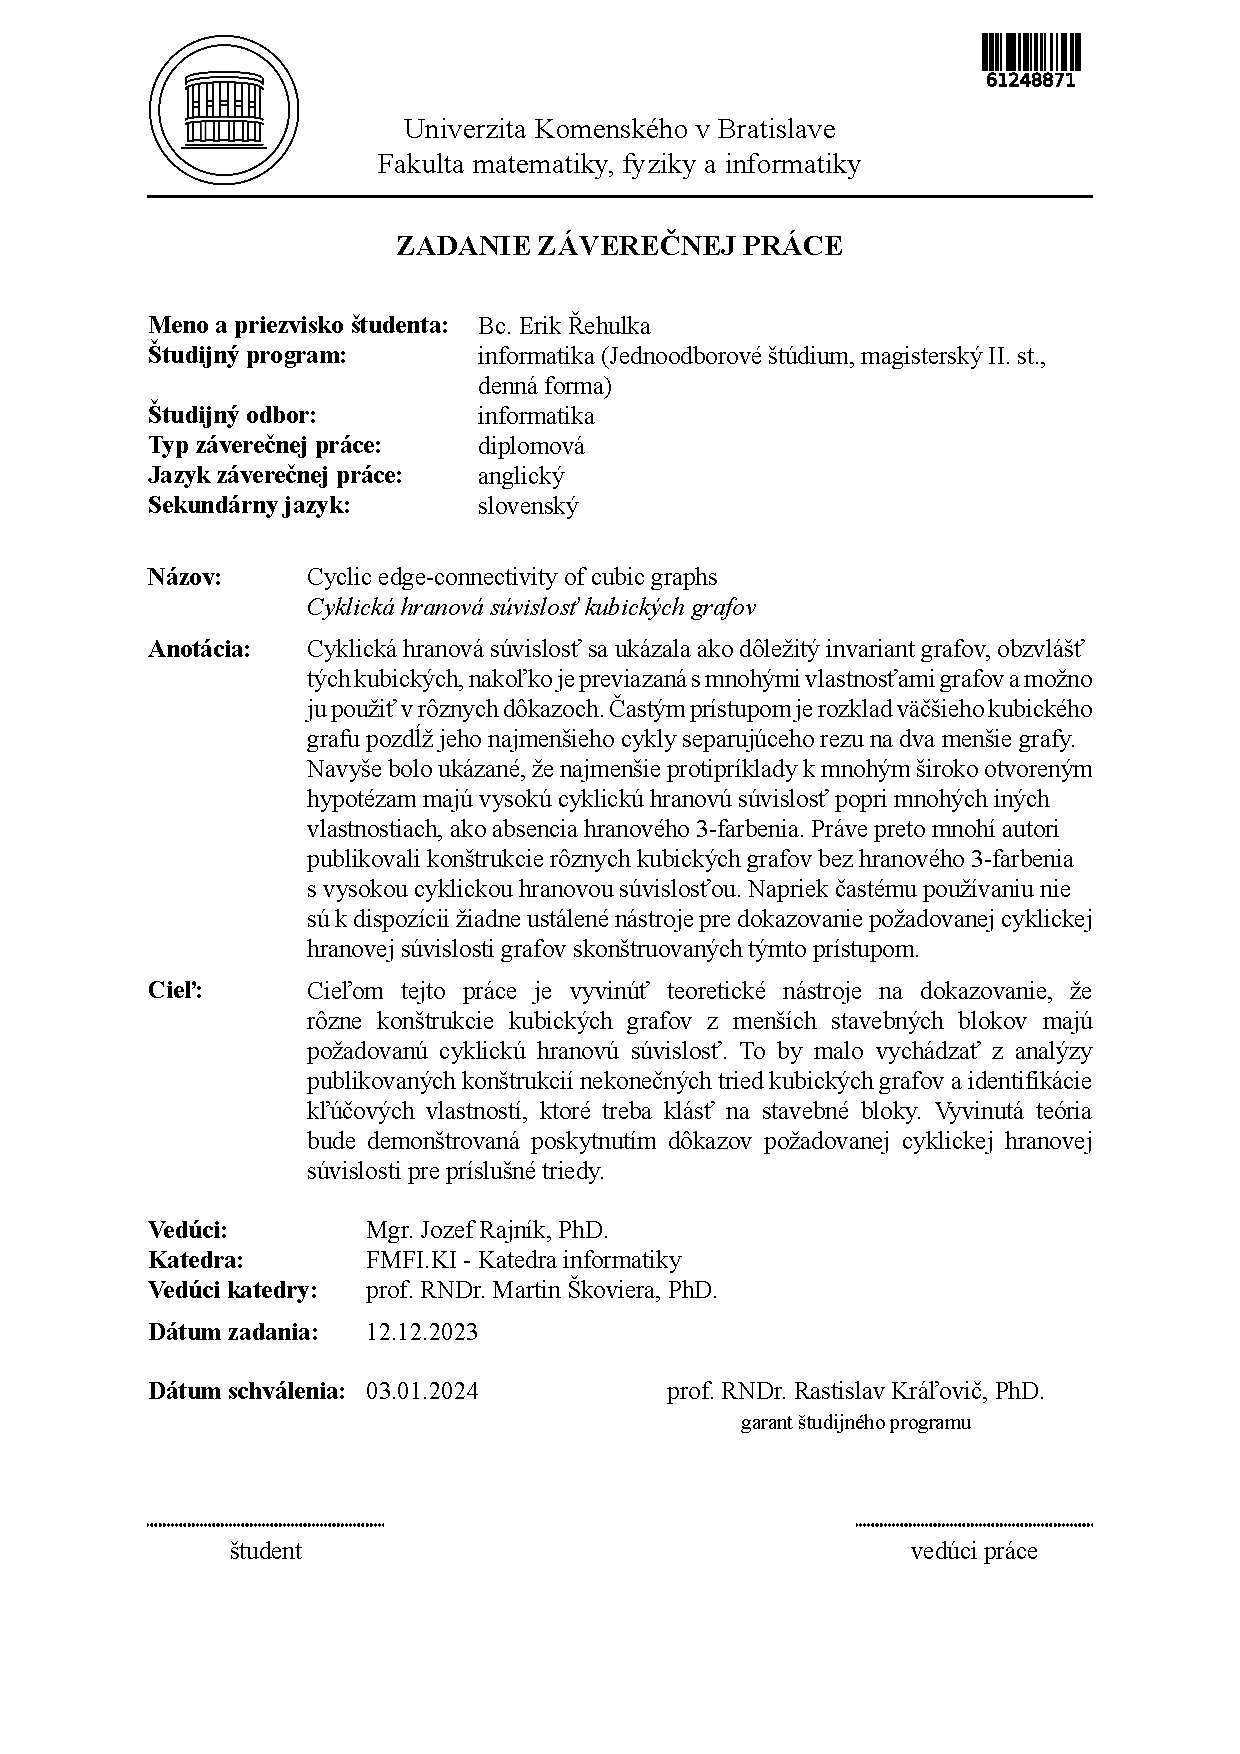
\includegraphics[trim=2.5cm 5cm 2.5cm 0,width=\textwidth]{images/assignment-sk.pdf}

\ifenglish{}
    \newpage
    \thispagestyle{empty}

    \noindent
    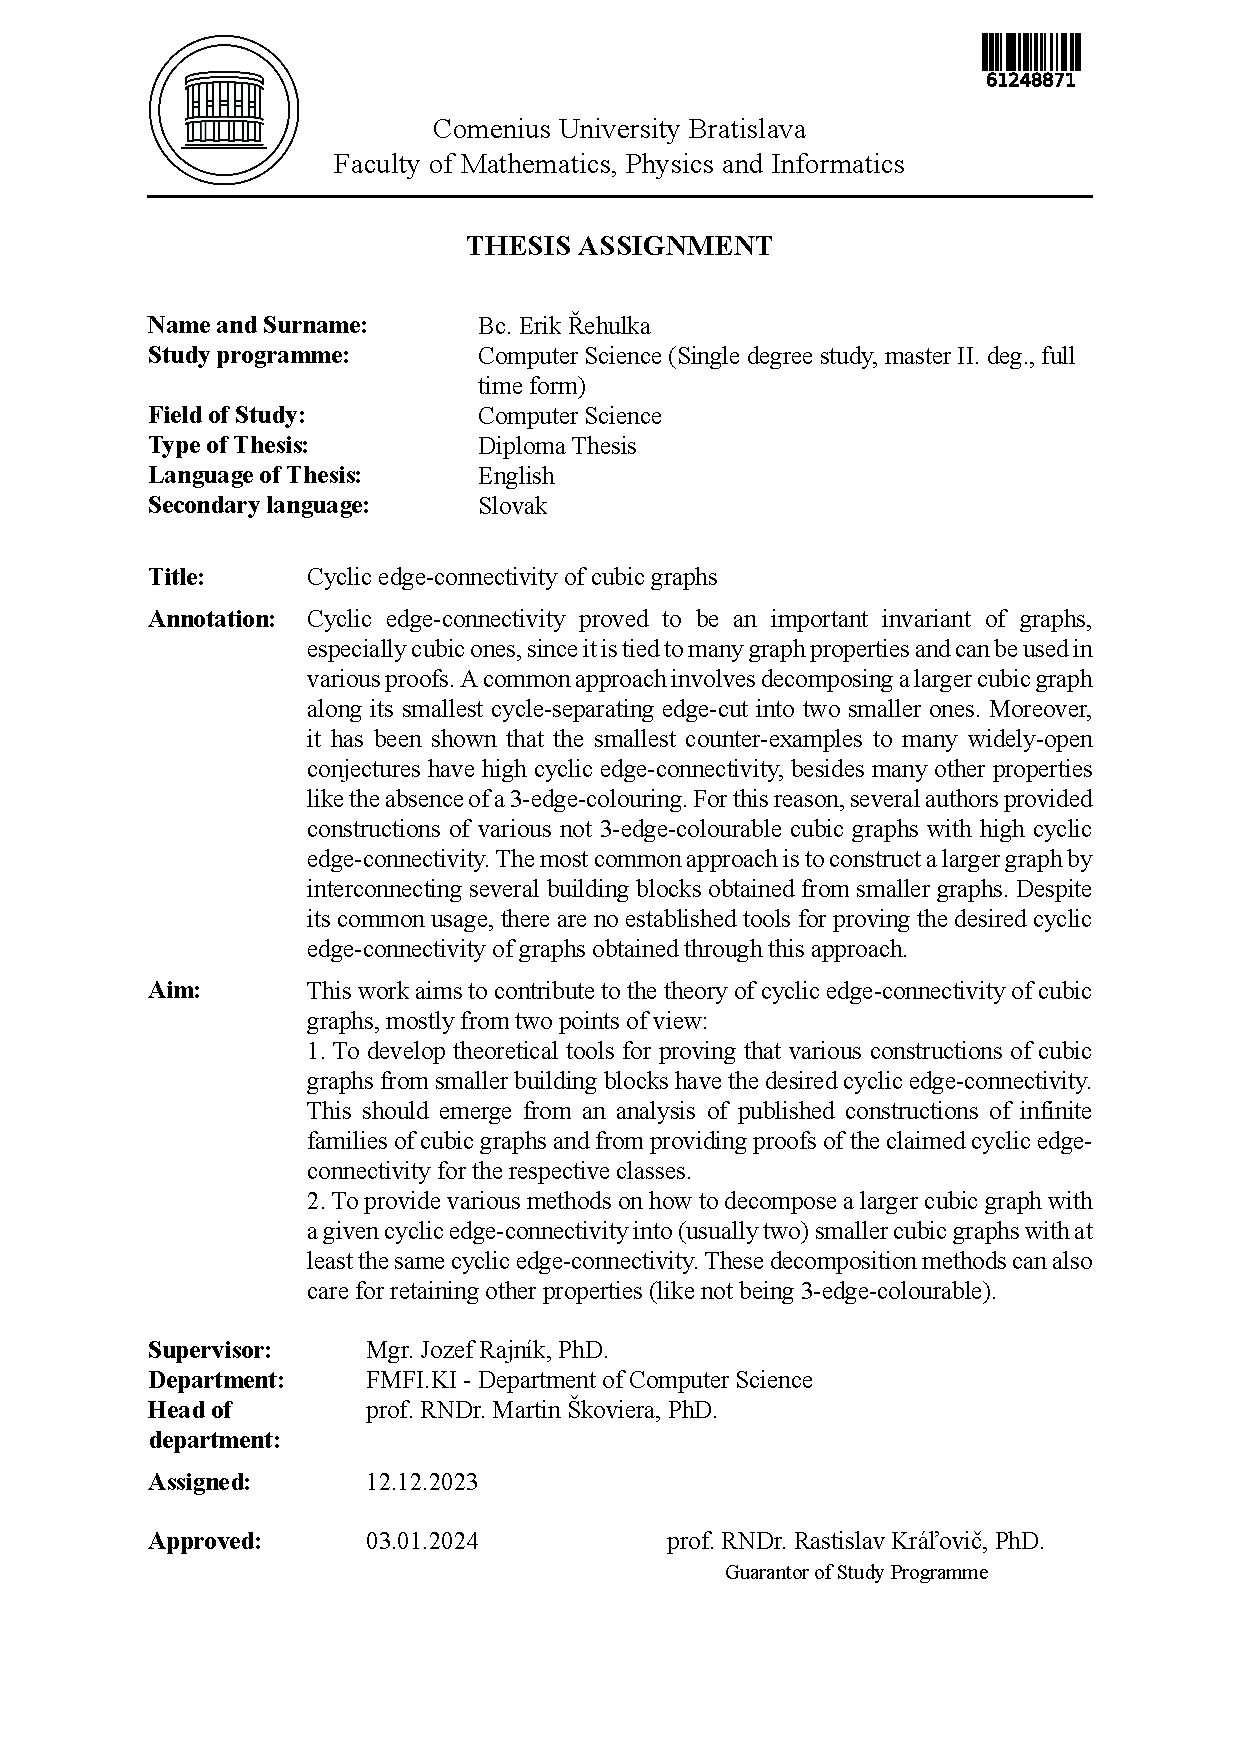
\includegraphics[trim=2.5cm 5cm 2.5cm 0,width=\textwidth]{images/assignment-en.pdf}
\fi

% ACKNOWLEDGEMENTS
\newpage

~\vfill
\paragraph*{\ifenglish{}Acknowledgments:\else{}Poďakovanie:\fi} \thesisacknowledgments{}

% ABSTRACT SK
\newpage

\begin{otherlanguage}{slovak}
    \section*{Abstrakt}

    \thesisabstractsk{}

    \paragraph*{Kľúčové slová:} \thesiskeywordssk{}
\end{otherlanguage}

% ABSTRACT EN
\newpage

\begin{otherlanguage}{USenglish}
    \section*{Abstract}

    \thesisabstracten{}

    \paragraph*{Keywords:} \thesiskeywordsen{}
\end{otherlanguage}

% TABLE OF CONTENTS, LIST OF FIGURES
\newpage
\tableofcontents

\newpage
\listoffigures

% CONTENTS
\mainmatter{}

\chapter*{Introduction}
\addcontentsline{toc}{chapter}{Introduction}
\markboth{Introduction}{Introduction}

\chapter{Preliminaries}\label{ch:preliminaries}

Definitions not provided in our work can be found in the book \quotes{Graph Theory} by Diestel \cite{Diestel}. All graphs considered in this work are undirected, connected and finite. We do not allow trivial graphs, but sometimes for the sake of complete definition we address them. We permit multiple edges, however loops are not allowed.

A \textit{girth} of a graph $G$, denoted by $g(G)$ is the minimum length of a cycle in $G$. If $G$ does not contain a cycle, we set the girth to $\infty$.

The distance between two vertices $x$ and $y$ in a graph $G$, denoted by $d_G(x,y)$, is defined as the length of the shortest path between $x$ and $y$ in $G$. If no such path exists, we set $d_G(x,y)=\infty$. If the specific graph $G$ is evident from the context, we shall only use $d(x,y)$.

While we work only with cyclic connectivity, for the sake of providing the definition completely in our work, we shall start with definining how we will compute connectivity, but more importantly, how we will work with edge cuts.

\section{Multipoles}\label{sec:multipoles}

In our work, we allow a specific type of graph, which allows ends of its edges to not be incident with a vertex, resulting in a graph with dangling, or even so-called isolated edges. Such structures are called \textit{multipoles}. This term was first used by Fiol in 1991 \cite{Fiol1991}, however we will be following a definition by Nedela and Škoviera \cite{Nedela1996}.

\begin{definition}[\cite{Nedela1996}]
	A \textit{multipole} is a pair $M=(V,E)$ of distinct finite sets of vertices $V$ and edges $E$, where every edge $e\in E$ has two edge ends, which may or need not be incident with a vertex.
	
	According to the incidence of edge ends, we define four types of edges:
	\begin{enumerate}[nolistsep]
		\item A \textit{link} is an edge whose ends are incident with two distinct vertices.
		\item A \textit{dangling edge} is an edge whose one end is incident with a vertex, and the other is not.
		\item An \textit{isolated edge} is an edge whose both ends are not incident with any vertex.
	\end{enumerate}
\end{definition}

A \textit{semiedge} is an edge end not incident with any vertex. For a given multipole $M$, we define $S(M)$ to be the tuple containing all the semiedges in that multipole. A set of all links in $M$ is denoted as $E_L(M)$.

A multipole $M$ with $n$ semiedges and $S(M) = (a_1, \cdots, a_n)$ can also be denoted as $M(a_1,\cdots,a_n)$. Similarly to graphs, the \textit{order} of a multipole $M$, denoted by $|M|$, is the number of its vertices. Also the \textit{degree} of a vertex $v$ of a multipole, denoted by $\deg(v)$, is the number of edge ends incident with $v$. A multipole with $k$ semiedges is usually called a \textit{k-pole}. It can be seen, that a graph can be defined as a 0-pole.

One of the features of multipoles is connecting them to form bigger multipoles or even graphs. They can be seen as small building blocks for constructing larger graphs or multipoles. 

Now, let $e$ and $f$ be edges (not necessarily distinct) and $e',~f'$ two of their semiedges respectively, such that $e'\neq f'$. If $e\neq f$, the result of the \textit{junction} of $e'$ and $f'$ is a new edge, having the other edge ends of $e$ and $f$ and a deletion of $e$ and $f$. If $e=f$, the result of the \textit{junction} of $e'$ and $f'$ is just the deletion of the edge.

Let $S=(e_1,\cdots,e_n)$ and $T=(f_1,\cdots,f_n)$ be two connectors, both with $n$ semiedges. The junction of two connectors $S$ and $T$ consists of $n$ individual junctions of semiedges $e_i$ and $f_i$ for $i$ from $1$ to $n$.

\todo{nechceme connectors! zbytočné}

The junction of two $(c_1,\cdots,c_n)$-poles $M(S_1,\cdots,S_n)$ and $N(T_1,\cdots,T_n)$ consists of $n$ individual junctions of connectors $S_i$ and $T_i$, for $i$ from $1$ to $n$. We denote the junction as $M(S_1,\cdots,S_n)*N(T_1,\cdots,T_n)$, or simply $M*N$ when we explain the connection. \todo{Možno nepotrebujeme tu ani tie connectors tbh. Definovať to môžeme cez bijekciu $f$ a $M*_f N$ resp. injekciu pri partial junction}

Consider two multipoles $M(a_1,\cdots,a_n)$ and $N(b_1,\cdots,b_m)$. Their \textit{partial junction} is a junction of some semiedges $(a_{i_1},\cdots, a_{i_k})$ and $(b_{j_1},\cdots, b_{j_k})$, where $k\leq n$ and $k\leq m$. In contrast to a normal junction, which results in a graph, the partial junction can still result in a multipole. 

\todo{prepis vsecko, nech to neni kopia bakalarky}

Similarly to the notion of subgraphs in graphs, we should define when a multipole is a \textit{submultipole} of another. A multipole $M$ is a submultipole of a multipole $N$ when there is a multipole $P$ and a partial junction $*$ such that $N=M*P$. In this case we say that $N$ contains $M$ as a submultipole.

\todo{definuj cyclic multipole/cyclic k-pole}

When we write some link $e$ as $xy$, we mean a link between vertices $x$ and $y$. On the other hand, when we just regard it as an edge $xy$, then $x$ and $y$ are its edge ends.

Since we allow these dangling and isolated edges, we can introduce so-called \textit{edge severing}. By severing an edge $e=e_1e_2$, we mean the removal of $e$, along with adding two new edges: $e_1e_3$ and $e_4e_2$, where $e_3$ and $e_4$ are new edge ends. It is evident that by severing a link we obtain two new dangling edges, by severing a dangling edge we obtain a new dangling edge and an isolated edge, and by severing an isolated edge we obtain two new isolated edges.

\section{Edge Cuts and Connectivity}\label{sec:edge-cuts}

As the name suggests, an \textit{edge cut} decomposes a graph into multiple connected components. It is a set of edges of a graph $G$, such that if we sever every edge in the set, the resulting graph will not be connected. There is also a second way to denote an edge cut, which is helpful when trying to determine how will the vertices be split after severing the edges. Note that by $E(V_1,V_2)$ we denote the set of edges, which have one end in $V_1$ and the other in $V_2$.

Let $G$ be a graph and ${V_1,V_2}$ a partition of $V(G)$, such that both sets are non-empty. By $E(V_1,V_2)$ we denote the set of edges, which have one end in $V_1$ and the other in $V_2$.

Note, that $E(V_1,V_2)$ is indeed an edge cut, when we sever all of these edges, there will not be any edge between a vertex in $V_1$ and $V_2$, splitting the graph into two components. The sets $V_1$ and $V_2$ are called the sides of the cut.

A graph which results from a graph $G$ by severing edges from a set $S$ is denoted as $G-S$. Note that this does not require $S$ to be an edge cut, the result can still be connected.

A graph $G$ is \textit{k-edge-connected} (for $k\in\mathbb{N}$), if $|G|>k$ and $G-S$ is connected for every set $S\subseteq E(G)$ such that $|S|<k$. In other words, there is no edge cut with less than $k$ edges.

\begin{definition}
	Let $G$ be a graph. The \textit{edge conectivity} of $G$, denoted by $\lambda(G)$ is the greatest $k\in\mathbb{N}$ such that $G$ is $k$-edge-connected.
\end{definition}

In other words, it is the size of the smallest edge cut in the graph. It can be easily proven, that for each non-trivial graph $G:~\lambda(G)\leq\delta(G)$, where $\delta(G)$ is the minimum degree. The proof comes from the fact, that all edges incident with a vertex are indeed edge cuts, separating the vertex from the rest of the graph, meaning there is an edge cut of size $\delta(G)$ in each graph.

\section{Cyclic Edge Connectivity}\label{sec:cyclic-edge-connectivity}

The latter can be a huge limitation, since for example when trying to explore cubic graphs, there is already an upper bound on the edge connectivity. Because of this, a new metrics regarding edge cuts were introduced, requiring both of the components resulting after severing edges from an edge cut to contain cycles. The notation is similar as before, just with a keyword \textit{cyclic} before it. To maintain a reasonable level of formalism, we shall define these properties more precise.

An edge cut $E(V_1,V_2)$ in a graph $G$ is called \textit{cycle separating}, if both induced subgraphs $G[V_1]$ and $G[V_2]$ contain a cycle. In contrast to edge cuts, there are non-trivial graphs which do not contain a cycle separating edge cut \cite{atoms-of-cyclic, Lou2008, lovasz1965graphs}, for example trees. 

Similarly to edge connectivity, we say that graph $G$ is \textit{cyclically k-edge-connected} (for $k\in\mathbb{N}$), if there is no cycle separating edge cut with less than $k$ edges.

\begin{definition}[\cite{atoms-of-cyclic}]
	Let $G$ be a graph. The \textit{cyclic edge conectivity} of $G$, denoted by $\zeta(G)$ is the greatest $k\in\mathbb{N}$ such that $G$ is cyclically $k$-edge-connected.
\end{definition}

If there is no cycle separating edge cut in a graph $G$, we say that $\zeta(G)=\infty$ \cite{Lou2008}.

\todo{Poriadnejšie definovať cyklickú k-časť, nech nie je viazaná na pôvodný graf}

More properties of cyclic edge connectivity are regarded in \cref{ch:cyclic-edge-connectivity}.

\section{Transitive graphs}\label{sec:transitive-graphs}

A graph $G$ is called vertex-transitive if for any two vertices $x,y\in V(G)$ there is an automorphism of $G$ mapping $x$ to $y$. Similarly, it is called edge-transitive if for any two edges \todo{dokonči korektne}

A vertex-transitive connected graph $G$ is called Cayley if it has a group $\Gamma$ of automorphisms such that for all $u, v \in V(G)$ there exists exactly one automorphism $\phi\in\Gamma$ such that $\phi(u)=v$. In other words, $\Gamma$ acts regularly on $V(G)$. The fact that there is a family of vertex-transitive graphs is very helpful for proving subsequent theorems, since cyclic-edge connectivity is interesting to explore on vertex-transitive graphs. For now we shall mention the following theorem about the existence of vertex-transitive graph with arbitrary girth and valence, which we will use to construct cubic vertex-transitive graphs.

\begin{theorem}[\cite{small-vertex-transitive}]\label{th:cayley-girth-valence}
	For every pair of parameters $k \geq 2, g \geq 3$, there exists a finite Cayley graph $C(\Gamma, X)$ of valence $k$ and girth $g$.
\end{theorem}

Thus there is a cubic vertex-transitive graph of arbitrary girth.

\chapter{Cyclic Edge Connectivity}\label{ch:cyclic-edge-connectivity}

As in other areas of graph theory, we may want to look for somewhat equivalent graphs in terms of a specific property, which are more simple (for example contain less vertices), but have the same value of the property as the original graph. When talking about cyclic edge connectivity, those are called \textit{reduced forms} and result from a graph by removing all of its trees, as mentioned in these lemmas. To be formally precise, when removing a vertex we also remove all of its incident edges, unless specified otherwise.

\begin{lemma}[{{\cite[Lemma 1]{Lou2008}}}]
	Let $G$ be a graph and let $v$ be a vertex of degree 1 in $G$. Then $\zeta(G-v)=\zeta(G)$.
\end{lemma}

By the repeated application of this lemma we get the following result.

\begin{lemma}[{{\cite[Lemma 2]{Lou2008}}}]
	Let $G$ be a graph with an edge cut of size 1. Let the only edge in this cut be $e=uv\in E(G)$. Let the component of $G-\{e\}$ connecting vertex $v$ be a tree $T$. Then $\zeta(G)=\zeta(G-T)$.
\end{lemma}

The tree $T$ from the latter lemma is called a \textit{pendant tree}. By the removal of each pendant tree in $G$ we obtain the mentioned reduced form $G'$ and the cyclic edge connectivity stays the same \cite{Lou2008}.

It is also possible to suppress a vertex of degree 2 in specific cases to not change the cyclic edge connectivity.

\begin{lemma}[{{\cite[Lemma 4]{Lou2008}}}]
	Let $G$ be a graph, let $x$ be a vertex of degree 2 in $G$ and let $xy, xz\in E(G)$. Let $G'$ be the graph obtained from $G$ by suppressing $x$. Then $\zeta(G')=\zeta(G)$ unless $G$ has a triangle $C=xyzx$. \todo{tu si pozri dôkaz poriadne, možno to neni úplne dobre}
\end{lemma}



% !!!! Toto asi nechceme použiť, len Betti number ako upper bound a spomenutie tých kubických grafov ktoré nemajú cycle separating cut !!!!!!
%
%\section{Infinite Cyclic Edge Connectivity}
%
%Graphs with infinite cyclic edge connectivity, in other words without a cycle separating edge cut, were already widely explored \cite{atoms-of-cyclic, Lou2008, lovasz1965graphs}. For cubic graphs, there are however not that many possibilities. As it comes from the following proposition, the only three possibilities are $K_4$, $K_{3,3}$ and $\Theta_2$, which is a graph consisting of two vertices and three parallel edges between them.
%
%\begin{proposition}[{{\cite[Proposition 1]{atoms-of-cyclic}}}]
%	A connected cubic graph $G$ has no cycle separating edge cut if and only if it is isomorphic to one of $K_4$, $K_{3,3}$, $\Theta_2$. In fact, if $C$ is a shortest cycle in $G$, then $E(C,V(G)-C)$ is a cycle separating edge cut unless $G$ is $K_4$, or $K_{3,3}$, or $\Theta_2$.
%\end{proposition}
%
%We say that two cycles $C_1$ and $C_2$ in a graph $G$ are independent if $V(C_1)\cap V(C_2) = \emptyset$. For arbitrary graphs, a rather obvious observation is that $\zeta(G)\neq\infty$ if and only if $G$ has two independent cycles.
%
%For graphs containing vertices of degree 1 and 2 (in other words graphs $G$ with $\delta(G)\leq 2$) we have already shown that it is possible to remove or suppress them and get a reduced form of $G$, which has the same cyclic edge connectivity as the original. For graphs with $\delta(G)\geq 3$ it is possible to describe when they have infinite cyclic edge connectivity.
%
%\begin{theorem}[{{\cite[Theorem 7]{Lou2008}}}]
%	Let $G$ be a connected graph with $\delta(G)\geq 3$ and $g(G)\geq 5$. Then $\zeta(G)\neq \infty$ if and only if $v(G)\geq 2g(G)$.
%\end{theorem}
%
%\todo{TU tie veci od Loua su celkom ze ocividne. Zaujimave je potom az tvrdenie Theorem 7}

\section{Cyclic parts}\label{sec:cyclic-parts}

\begin{proposition}[{{\cite[Proposition 2]{atoms-of-cyclic}}}]\label{prop:cyclic-con-less-than-girth}
	For every connected cubic graph $G$ it holds that $\zeta(G)\leq g(g)$.
\end{proposition}

\begin{lemma}[{{\cite[Lemma 5.1]{Rajnik_phd}}}]\label{lem:rajnik5.1}
	Let $M$ be an $s$-pole with girth at least $k$ different from a $k$-cycle for some $s\leq k$. Then $|M| \geq 2k - 4$.
\end{lemma}

\begin{theorem}[{{\cite[Theorem 17]{atoms-of-cyclic}}}]\label{th:cyclic-connectivity-of-transitive}
	Let $G$ be a cubic vertex-transitive or edge-transitive graph of girth $g$. Then $G$ has no non-trivial proper atom. In particular, $\zeta(G) = g$.
\end{theorem}

\section{Algorithms}\label{sec:algorithms}

In this chapter we provide known algorithms to determine cyclic edge connectivity of graphs. It is a long standing problem, whether to determine cyclic edge connectivity of an arbitrary graph is in $P$ \todo{zdroj?}. However, there are several polynomial algorithms for determining the cyclic edge connectivity of graphs with some specific attributes.

\chapter{Formulation of our problems}\label{ch:problem-formulation}

In this chapter we introduce the problems investigated in this thesis, along with a motivation and goals we want to fulfill. In the end we provide the main results from given problem.

\section{Cyclic Edge Connectivity of junctions of cubic cyclic $k$-parts}

\section{Cyclic edge connectivity of cubic graph decompositions}


\chapter{Results}\label{ch:results}

\section{Cyclic parts}\label{sec:cyclic-part-results}

We denote the $k$-pole, which is the $k$-cycle where each vertex is incident with one dangling edge as $C_k$.

\begin{lemma}\label{lem:each-cycle-cyclic-part}
	For each $k\geq 1$ the $k$-pole $C_k$ is a cyclic $k$-part. 
\end{lemma}

\begin{proof}
	For given $k$ we can construct a cubic Cayley graph with girth $k$ according to \cref{th:cayley-girth-valence}. Let us denote this graph as $G_k$. Then $\zeta(G_k)=k$ by utilizing \cref{th:cyclic-connectivity-of-transitive}. Since the girth of $G_k$ is $k$, it contains a cycle of length $k$ and thus $G_k=C_k*P$ for some other $k$-pole $P$. It is evident that if $P$ contains a cycle, the edge cut $E(V(C_k), V(P))$ in $G_k$ is cycle-separating and since $|E(V(C_k), V(P))|=k$ (both are $k$-poles) $C_k$ is a cyclic $k$-part.
	
	We prove that the $\delta(P)=2$, this leads to proving $P$ contains a cycle. Suppose $\delta(P)<2$, this would mean that there is a vertex in $P$ incident with more than one dangling edge. Say these two dangling edges are $e',f'$. Then in $G_k$ these are junctioned with some dangling edges in $C_k$, let $X$ be the shortest path between these dangling edges in $C_k$. We see that $|X|<\frac{k}{2}$ since $C_k$ is a cycle. Let $e,f$ be the links in $G_k$ resulting from the junction of $C_k$ and $P$ such that $e$ resulted from a junction of two dangling edges containing $e'$ and $f$ from a junction containing $f'$. Then there is a cycle $eXf$ in $G_k$ of length smaller than $\frac{k}{2}+2$. The girth of $G_k$ is $k$ thus $k<\frac{k}{2}+2$, leading to the fact that $k<4$. This leads to a contradiction for $k\geq 4$, however we need to prove that $C_1,C_2$ and $C_3$ are in fact cyclic $k$-parts.
	
	\begin{figure}
		\centering
		\begin{subfigure}[c]{0.3\textwidth}
			\centering
			\begin{tikzpicture}[scale=0.8, baseline]
				% First graph (dumbbell)
				\node[draw, circle] (a1) at (0,0) {};
				\node[draw, circle] (b1) at (2,0) {};
				\draw (a1) -- (b1);
				\draw (-1,0) circle [radius=1];
				\draw (3,0) circle [radius=1];
				\draw [dashed] (1,1.5) -- (1,-1.5);
			\end{tikzpicture}
		\end{subfigure}%
		\begin{subfigure}[c]{0.3\textwidth}
			\centering
			\begin{tikzpicture}[scale=0.8, baseline]
				% Second graph (two vertices on each side)
				\node[draw, circle] (a1) at (0,1) {};
				\node[draw, circle] (a2) at (0,-1) {};
				\node[draw, circle] (b1) at (2,1) {};
				\node[draw, circle] (b2) at (2,-1) {};
				\draw (a1) -- (b1);
				\draw (a2) -- (b2);
				\draw (a1) to[bend left] (a2);
				\draw (a1) to[bend right] (a2);
				\draw (b1) to[bend left] (b2);
				\draw (b1) to[bend right] (b2);
				\draw [dashed] (1,1.5) -- (1,-1.5);
			\end{tikzpicture}
		\end{subfigure}%
		\begin{subfigure}[c]{0.3\textwidth}
			\centering
			\begin{tikzpicture}[scale=0.7, baseline]
				\begin{scope}
					\graph[clockwise, radius=1cm, empty nodes] {subgraph C_n [n=3,name=A] };
				\end{scope}
				\begin{scope}[xshift=4cm]
					\graph[clockwise, radius=1cm, empty nodes] {subgraph C_n [n=3,name=B] };
				\end{scope}
				\draw (A 1) -- (B 1);
				\draw (A 2) -- (B 3);
				\draw (A 3) to[bend right] (B 2);
				\draw [dashed] (2,2) -- (2,-3);
			\end{tikzpicture}
		\end{subfigure}
		\caption{Junctions (marked by the dashed lines) $C_1*C_1, C_2*C_2$ and $C_3*C_3$}
		\label{fig:C1C2C3_junctions}
	\end{figure}
	
	As seen in \cref{fig:C1C2C3_junctions} by performing an arbitrary junction $C_i*C_i$ we obtain a graph with $\zeta(C_i*C_i)=i$ for each $i\in \{1,2,3\}$. This proves that for each $k\geq 1$ the $k$-pole $C_k$ is a cyclic $k$-part.
\end{proof}

\begin{lemma}\label{lem:cyclic-part-no-small-submultipole}
	Let $P$ be a cyclic $k$-part. Then for each $l<k$ it holds that $P$ does not contain a cyclic $l$-pole as a submultipole.
\end{lemma}

\begin{proof}
	Suppose by contradiction that $P$ contains a cyclic $l$-pole $Q$ as a submultipole, where $l<k$. Let $R$ be the other multipole for which $P=Q*_fR$ for some injection $f:S(Q)\rightarrow S(R)$. Since $P$ is a cyclic $k$-part, there is a graph $G$ with $\zeta(G)=k$ which is a junction of $P$ and some other cyclic $k$-part $P'$, thus $G=P*_gP'$ for some injection $g:S(P)\rightarrow S(P')$. Let $E$ be the set of links of $G$, which result from the partial junctions $*_f$ and $*_g$ and one of the junctioned semiedges is from $S(Q)$. We see that $E$ is an edge cut separating $G$ into $Q$ and $R*_gP'$, let us denote the second multipole as $T$. Since $Q$ is cyclic and $P'$ as well, implying $T$ is also cyclic, $E$ is cycle separating. From the definition of $E$ we see that $|E|=|S(Q)|$ and since $|S(Q)|=l$, we have found a cycle separating edge cut with less than $k$ edges in $G$, leading to a contradiction.
\end{proof}

From this we can construct one corollary, which will be useful in proving subsequent theorems.

\begin{corollary}
	Let $M$ be a cyclic $k$-part. Then there is no edge cut $S$ of size $l$ separating $M$ into two multipoles $M_1$ and $M_2$ such that $M_1$ contains a cycle and $k_1$ semiedges from the former $k$-pole $M$, for which $l+k_1 < k$.
\end{corollary}

\begin{proof}
	Let $G$ be a cubic graph with $\zeta(G)=k$ such that $G=M*N$ for some cyclic $k$-part $N$. We know that at least one of these graphs exists, since $M$ is a cyclic $k$-part. Suppose that there would be such edge cut $S$ of size $l$ in $M$ separating it into two multipoles $M_1$ and $M_2$ such that $M_1$ contains a cycle and $k_1$ semiedges from $M$ and $l+k_1 < k$. This would however mean that $M$ contains a cyclic $(l+k_1)$-pole $M_1$, contradicting \cref{lem:cyclic-part-no-small-submultipole}.
\end{proof}

% Toto je podľa mňa príliš zložito spísaný dôkaz toho pred tým, asi to nepotrebujeme, len potom to treba správne použiť v dôkaze kde sa to používalo.
%
%\begin{lemma}
%	\label{lem:cyclic-part-no-short-cut}
%	Let $P$ be a cyclic $k$-part. Let $S$ be an edge cut separating $P$ into two components $P_1$ and $P_2$ such that $P_1$ contains a cycle. Then it holds that ${|S| \geq |S(P)\cap S(P_2)|}$.
%\end{lemma}
%
%\begin{proof}
%	Note that $S(P)\cap S(P_i)$ contains all of the semiedges from $P$, which are in $P_i$ after cutting the edges, for both $i\in\{1,2\}$.
%	
%	Let $G$ be a cubic graph with cyclic edge-connectivity $k$ and let $S_G$ be a cycle-separating $k$-edge-cut such that one of the cyclic $k$-parts of $G-S_G$ is $P$. Let us denote the other cyclic $k$-part by $Q$. Suppose that there is such edge cut $S$, for which it holds that $|S| < |S(P)\cap S(P_2)|$. 
%	
%	When severing an edge $e$, let the new created semiedges be denoted as $e_1$ and $e_2$. For $i\in\{1,2\}$ denote by $E_i$ the set of edges such that $$E_i=\{e ~|~ e\in S_G, \exists i \in \{1,2\}: e_i\in S(P_i)\}$$
%	
%	so edges from $S_G$, for which after their severing, one of the new created semiedges is in $P_i$. We prove that $S_G=E_1\cup E_2$. Since $E_i\subseteq S_G$ for both $i\in\{1,2\}$, it is evident that $E_1\cup E_2\subseteq S_G$. For each edge in $S_G$, one of the resulting semiedges is in $P$ and the other in $Q$. Suppose otherwise, so there is an edge $e$, for which both resulting semiedges are in one of $P$ or $Q$. Without loss of generality, let both be in $P$. Then $S_G-\{e\}$ is a cycle-separating edge-cut in G with $k-1$ edges, contradicting the fact that $G$ is cyclically $k$-edge-connected. Since from each edge $f\in S_G$ one of the resulting semiedges is in $P$, say $f_1$, it must be in $P_1$ or $P_2$, thus $S_G\subseteq E_1\cup E_2$.
%	
%	Note that $S\cup E_1$ is an edge-cut in $G$, separating it into components $P_1$ and a partial junction of $P_2$ and $Q$. By assumption $P_1$ contains a cycle and $Q$ is a cyclic part, thus also contains a cycle, which means that $S\cup E_1$ is cycle-separating.
%	
%	We prove that $|S(P)\cap S(P_2)|=E_2$. Since $E_2$ contains all edges from $S_G$, which create a semiedge in $S(P)\cap S(P_2)$, it holds that $|E_2|\leq |S(P)\cap S(P_2)|$. For the other inequality, we see that all semiedges in $S(P)\cap S(P_2)$ were created by the cut $S_G$, specifically by its subset $E_2$. Each edge from $E_2$ creates only one such semiedge. Suppose the contrary, so there would be some edge $e\in E_2$, for which both semiedges $e_1$ and $e_2$ would be in $P_2$. It is evident that $S_G-\{e\}$ is a cycle-separating edge-cut in $G$ with $k-1$ edges, contradicting the fact that $G$ is cyclically $k$-edge-connected. Because of this $|S(P)\cap S(P_2)|\leq |E_2|$. 
%	
%	Note, that $|S| < |E_2|$, since $|S| < |S(P)\cap S(P_2)|$ and $|S(P)\cap S(P_2)|=|E_2|$. It holds that $S\cap E_1=\emptyset$, since $S$ is an edge cut in $P$ and there are no edges left in $P$ from $E_1$, as each of them was severed when creating $P$. Also $E_1\cap E_2=\emptyset$. Suppose the contrary, so there would be some edge $e$ which is in $E_1$ and $E_2$. This would mean that both of its incident vertices would be in $P$, which contradicts the assumption that $G$ is cyclically $k$-edge-connected, as we have proved above. However, this would mean that $|S\cup E_1|< |E_1\cup E_2| = |S_G|=k$, thus $S\cup E_1$ is a cycle-separating cut with at most $k-1$ edges, contradicting the assumption that $G$ is cyclically $k$-edge-connected.
%	
%	\todo{uviesť ilustrácie}
%\end{proof}


\begin{theorem}\label{th:junction-of-kpoles-cyclic-edge-connectivity}
	Let $M_1$ and $M_2$ be cyclic cubic $k$-poles such that neither contains a cyclic $l$-pole as a submultipole for $l<k$. Let both $M_1$ and $M_2$ be different from the cycle of length $k$ or $k\leq 5$. Let $G$ be the junction of $M_1$ and $M_2$. Then $\zeta(G)=k$ unless the girth of $G$ is smaller than $k$.
\end{theorem}

\begin{proof}
	Let us denote the $k$-cut obtained after the junction $M_1*M_2$ by $S$. Suppose by contradiction that $G$ has girth at least $k$ and contains a cycle separating edge cut $T$ of minimal size, such that $|T|=l<k$ and it separates $G$ into two components $X_1$ and $X_2$. Note that in this case $\zeta(G)=l$. Let $A_1,A_2,A_3,A_4$ denote the subgraphs of $G$ induced by $V(X_1)\cap V(M_1), V(X_1)\cap V(M_2), V(X_2)\cap V(M_2), V(X_2)\cap V(M_1)$ respectively. Let $a,b,c,d,e$ and $f$ denote the number of edges connecting $A_1$ and $A_2$, $A_1$ and $A_3$, $A_1$ and $A_4$, $A_2$ and $A_4$, $A_3$ and $A_4$, $A_2$ and $A_3$ respectively as seen in \cref{fig:rajnik-cyclic-part-junction-illustration}.
	
	\begin{figure}
		\centering
		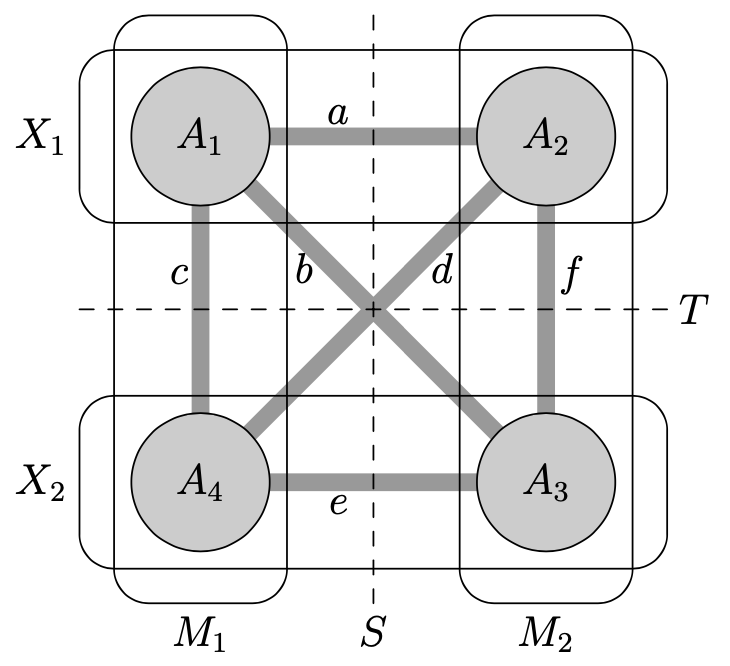
\includegraphics[width=0.5\linewidth]{graphs/rajnik-cyclic-part-junction-illustration}
		\caption{\cite{Rajnik_phd} Intersecting cuts S and T in the graph G}
		\label{fig:rajnik-cyclic-part-junction-illustration}
	\end{figure}
	
	Next let $r_i=|\delta(A_i)|$ for each $i\in\{1,2,3,4\}$. We can see that each of such $r_i$ is determined by the values of $a,b,c,d,e$ and $f$, for instance $r_1=a+b+c$. We prove by contradiction that each of $A_1, A_2,A_3$ and $A_4$ is non-empty. Suppose that some $A_i$ for $i\in\{1,2,3,4\}$ is empty. Then $M_1$ or $M_2$ would contain the whole cyclic $l$-pole $X_1$ or $X_2$, contradicting the assumption about $M_1$ and $M_2$.
	
	From the sizes of $S$ and $T$ we know that
	\begin{align}
		a+b+d+e &= k, \label{abde_eq_k}\\
		l=c+b+d+f &< k. \label{cbdf_smaller_k}
	\end{align}
	
	We now show that for each $i\in\{1,2,3,4\}$ at least one of the inequalities $r_i\geq k$ or $r_{i+1}\geq k$ is true, taking the indices modulo 4. Suppose to the contrary that there exists such $i\in\{1,2,3,4\}$ for which $r_j\leq k-1$ for both $j\in\{i, i+1\}$. Let us look at the properties of one of such $A_j$. We know that it contains less than $k$ semiedges, say $m$. We prove that is must be acyclic by contradiction. Let $A_j$ be in $M_1$, the proof for $M_2$ is analogous. Suppose that it would contain a cycle. Then $A_j$ would be a cyclic $m$-pole with $m<k$, contained in $M_1$, contradicting the assumption about $M_1$. Thus, we have that $|A_j|\leq r_j-2\leq k-3$ for both $j\in \{i, i+1\}$. By denoting $M$ as $G[A_i\cup A_{i+1}]$ we have $|M|\leq 2k-6$ ($A_i$ and $A_{i+1}$ are vertex disjoint). Note that $M$ is by its definition one of the multipoles $X_1, X_2, M_1,$ or $M_2$. This means that $M$ is cyclic and $|M|\geq k$ due to the girth of $G$ which must be at least $k$. From $k\leq |M|\leq 2k+6$ we have $k\geq 6$ so by the assumption of the theorem $M_1$ and $M_2$ are different from the $k$-cycle. Also both of $X_1$ and $X_2$ are different from $k$-cycles since they have less than $k$ semiedges. Therefore $M$ is not a $k$-cycle and it is a cyclic multipole with at most $k$ semiedges and girth at least $k$, so by \cref{lem:rajnik5.1}, $|M| \geq 2k - 4$, contradicting the fact that $|M|\leq 2k-6$.
	
	Thus for each $i\in\{1,2,3,4\}$ we have $r_i\geq k$ or $r_{i+1}\geq k$, from which it follows that
	\begin{align}
		r_1 =a+b+c\geq a+b+d+e=k \text{ and } r_3 =b+e+f \geq a+b+d+e=k\label{r1r3}
	\end{align}
	
	or
	\begin{align}
		r_2 =a+d+f \geq a+b+d+e=k \text{ and } r4 =c+d+e\geq a+b+d+e=k\label{r2r4}
	\end{align}
	
	is true. After summing, Inequalities \cref{r1r3} imply that $c+f\geq a+2d+e\geq a+e$ and Inequalities \cref{r2r4} imply that $c+f\geq a+2b+e\geq a+e$. In both cases we have obtained $c+f\geq a+e$. However by Inequality \cref{cbdf_smaller_k} we have 
	$$l=b+c+d+f<a+b+d+e=k$$
	
	so $c+f<a+e$, leading to a contradiction.
	
	We see that there is no cycle separating edge cut in $G$ with less than $k$ edges. Also there is the cycle-separating $k$-edge-cut $S$, thus it must be minimal and $\zeta(G)=k$.
	
	If the girth of $G$ would be less than $k$, then $\zeta(G)<k$ as well, because of \cref{prop:cyclic-con-less-than-girth}.
\end{proof}

A corollary of this theorem is that in this case the cyclic $k$-poles $M_1$ and $M_2$ are cyclic $k$-parts.

If we would be able to construct a cyclic $k$-pole for each $k$, such that it contains a cycle, has girth at least $k$ and does not create short cycles when connected to another cyclic $k$-pole, we could make it easier to decide if given cyclic $k$-pole is a cyclic $k$-part. If it does not contain a cyclic $l$-pole such that $l<k$, the \cref{th:junction-of-kpoles-cyclic-edge-connectivity} can be applied and thus it would be a cyclic $k$-part. However we first need to find such cyclic $k$-poles for each $k$. \todo{spomeň asi nejak adjuncts}

\todo{výraz submultipole nechceme používať, skôr že čo znamená keď graf obsahuje (contains) nejaký multipól}

\begin{lemma}\label{lem:cyclic-k-pole-no-short-cycles-exists}
	For each $k\geq 1$, there exists a cyclic $k$-pole with the following properties:
	\begin{enumerate}
		\item The girth is at least $k$,
		\item It contains no cyclic $l$-pole for any $l<k$,
		\item The distance between any pair of semiedges is at least $k-2$.
	\end{enumerate}
\end{lemma}

\begin{proof}
	For $k$ equal to 1 and 2 we see that $C_k$ fulfills the requirements, we shall only explore $k\geq 3$. For given $k$ we construct a cubic Cayley graph with girth $2k$ according to \cref{th:cayley-girth-valence}. Let us denote this graph as $G$. Then $\zeta(G)=2k$ by utilizing \cref{th:cyclic-connectivity-of-transitive}. Next let $P$ be a path of length $k-3$ in $G$. Since $k\geq 3$ and $|V(G)|$ is evidently at least $2k$, there will always be such path. Remove all of the vertices on this path and denote the result as $G'$. Since by removing some vertices and edges from a graph it is not possible to lower a girth, or introduce a new smaller cyclic $l$-pole, we must prove only the third condition about the distance between the semiedges. To be precise, we need to prove that
	\begin{enumerate}
		\item $G'$ is a cyclic $k$-pole,
		\item the distance between any pair of semiedges in $G'$ is at least $k-2$.
	\end{enumerate}
	The latter is easier to prove. \todo{dokonci}
	
	\todo{ilustrácia}
\end{proof}

We will denote the cyclic $k$-poles constructed this way as $W_k$.

\begin{theorem}\label{th:alternative-definition-of-cyclic-part}
	Let $M$ be a cyclic cubic $k$-pole such that it contains no cyclic $l$-pole for any $l<k$. Then $M$ is a cyclic $k$-part.
\end{theorem}

\begin{proof}
	Since each $k$-cycle $C_k$ is a cyclic part as proven in \cref{lem:each-cycle-cyclic-part} we can assume that $M$ is different from a cycle. Let $W_k$ be a cyclic $k$-pole satisfying \cref{lem:cyclic-k-pole-no-short-cycles-exists} and let $G$ be a junction $M*W_k$. We prove that $G$ has girth at least $k$. Suppose by contradiction that $g(G)<k$. Let us denote the shortest cycle in $G$ as $C$, $|C|=l\leq k-1$. There are multiple possibilities of where the cycle is located, we shall explore all of them.
	\begin{enumerate}
		\item $C$ is contained in $M$. Since $|C|=l$ and $M$ is cubic, $M$ contains the $l$-pole $C_l$ as well, contradicting the assumption.
		\item $C$ is contained in $W_k$. This leads to a contradiction, since we have constructed $W_k$ in a way that it has girth at least $k$.
		\item $C$ is not contained in neither, instead it was created after the junction $M*W_k$. Let the cycle be $ePfQ$, where $e$ and $f$ are edges resulting from the junction $M*W_k$, $P$ are edges inside $W_k$ and $Q$ is the rest of the edges of the cycle. However since the distance of any two semiedges in $W_k$ is at least $k-2$, it holds that $|P|\geq k-2$ and thus $|ePf|\geq k$, contradicting the fact that the cycle is shorter than $k$.
	\end{enumerate}

	Since all cases lead to a contradiction it holds that $g(G)\geq k$. Thus we see that $G$ is a cyclic cubic graph with girth at least $k$, resulting from the junction $M*W_k$. Since both $M$ and $W_k$ do not contain a cyclic $l$-pole for $l<k$, both are different from a cycle of length $k$ and their junction $G$ has girth at least $k$, we can apply \cref{th:junction-of-kpoles-cyclic-edge-connectivity} and conclude that $\zeta(G)=k$. Because of this fact we have proved that $M$ is in fact a cyclic $k$-part.
\end{proof}

\todo{Zamyslenie nad algoritmom na zisťovanie/generovanie cyklických častí}

Potencially cyclically k-connected:
\begin{itemize}
	\item Neobsahuje cyklický $l$-pól pre $l<k$.
\end{itemize}

\begin{theorem}
	Let $M_1$ and $M_2$ be potencially cyclically $k$-connected multipoles with the same number of semiedges. Let $m_i$ be the size of the smallest edge cut in $M_i$ such that one of the components contains at least 2 semiedges from $M_i$. If $m_1,m_2>1$ and $m_1+m_2\geq k$ then the partial junction $M=M_1*M_2$ is potencially cyclically $k$-connected unless $M$ has less than $k$ semiedges.
\end{theorem}

\begin{proof}
	Notes:
	\begin{itemize}
		\item Contradiction - there is an $l$-pole $X$ with $l<k$.
		\item $A_1,\cdots$ same as before, however $x_i$ equals semiedges from $A_i$.
		\item We prove that $M-X$ contains a cycle. We can easily prove that it is non-empty, thus contains some parts from $M_1$ or $M_2$. TODO NOT SO EASY! Possible fix - change the definition of potentially cyclically $k$-connected to not containing such $l$-pole $X$, that $G-X$ contains a cycle. This should not disrupt the equivalence in graphs between potentially cyclically connected and cyclically connected.
		
		Former notes: This should be from the fact that it is an independent edge cut and if there are vertices with degree 1 or 0 in $M-X$ we can modify the cut for it to have the same length or less.
		\begin{enumerate}
			\item If there is a vertex with degree 0, we have cut at least 2 of the edges incident with the vertex. This should lead to a contradiction with the cut being independent.
			\item If there is a vertex with degree with degree 1, there are multiple possibilities. We cut 2 edges, 1 edge, or none. If we cut 2, it should lead to a contradiction with the fact that the cut is independent. If we cut none, it would violate the condition of $m_i>1$ (the vertex has two dangling edges). If we cut one, then TODO.
		\end{enumerate}
		\item We shall prove that all $A_i$ are non-empty. $A_1$ and $A_2$ are easy, otherwise the whole $l$-pole is in $M_1$ or $M_2$.
		\item $A_3$ and $A_4$ can't be empty in the same time because $M$ has $k$ or more semiedges.
		\item If $A_3$ is empty, then the whole $M_2$ is contained in $X$. We then prove that $M-X$ is a cyclic $j$-pole with $j\leq l < k$, and contained in $M_1$ leading to a contradiction. We know that $M-X$ has a cycle, and number of its semiedges is in this case $c+d+x_4$, since $A_3$ is empty. also we know that $x_1+x_2=x_3$ since $M_1$ and $M_2$ have the same number of semiedges. We then know that $c+b+d+f+x_1+x_2<k$, from what we can see that $c+d+x_4<k$. Same goes for empty $A_4$.
		\item Then we must prove that $a$ is at least 2. If it was 0, then there would be a cyclic pole with less than $l$ semiedges in $M_1$ or $M_2$. If it was 1, then the whole cycle would be in $A_1$ or $A_2$. Suppose it is in $A_1$. We know that $c+b+d+f+x_1+x_2<k$. $a=1$, thus $a\leq k$ and $c+b+d+a+x_1+x_2<k$. From this we see that $a+b+c+x_1<k$, meaning there would be a cyclic $j$-pole with $j<k$ in $M_1$, leading to a contradiction.
		\item Because of this $c$ and $f$ must hold that $c+f\geq k$. They are cuts in $M_1, M_2$ because all $A_i$ are non-empty and they are connected components (TODO - should we say that in the theorem that they must be connected?). This leads to a contradiction with the fact that $c+b+d+f+x_1+x_2=l<k$.
	\end{itemize}
\end{proof}

PROBLEMS:

Momentálne berieme ako $m_i$ najmenší rez, kde jeden z komponentov má aspoň 2 polhrany pôvodného. To je ale vždy zhora ohraničené 3, bude to treba zovšeobecniť. Napríklad, že ten druhý komponent musí obsahovať cyklus alebo aspoň 2 polhrany? Respektíve 1 polhranu?

Potom by sme museli pridať pred posledným krokom aj dôkaz, že $A_4$ má cyklus, alebo $e+d+x_4\geq 1$ a rovnako pre $A_3$ (alebo 2)? 


\section{Cyclic part inflations}\label{sec:cyclic-part-inflations}

\begin{definition}[{{\cite[Definition 10]{HISTs}}}]
	Let $G$ be a graph and let $H$ be a cubic graph. Then $H$ is called an inflation of $G$ if $H$ contains a 2-factor $F$ consisting of chordless cycles such that the graph obtained from $H$ by contracting each cycle of $F$ to a vertex is isomorphic to $G$. By $I(G)$ we denote the set of all inflations of $G$.
\end{definition}

Informally speaking, one can obtain an inflation of $G$ by expanding each of its vertices to a cycle with the length same as the degree of the respective vertex in $G$. We can extend this definition, by allowing expanding each vertex of the original graph into a cyclic $k$-part, where $k$ is the degree of the respective vertex.

\todo{Definovať kedy vrcholy korešpondujú cyklickej časti v grafe, teda keď pospájam cyklické časti $P_1,\cdots, P_n$ do výsledku $G$, tak kedy nejaká množina vrcholov $V$ korešponduje v $G$ s $P_i$. Resp. treba to definovať?}

Let $G$ be a graph and $V$ a subset of its vertices. By \textit{contracting} $V$ in $G$ we obtain a new graph $G'$, such that:
\begin{itemize}
	\item For the vertices of $G'$ it holds that $V(G') = (V(G)-V)\cup \{v\}$ where $v$ is a new vertex.
	\item Let $E$ be a set containing such edges from $G$, which are incident with one vertex in $V$ and one in $V(G)-V$. Formally, ${E=\{xy~|~xy\in E(G), x\in V, y\notin V\}}$. Let $E'$ be a set of edges, which are incident with two vertices from $V$, formally ${E'=\{xy ~|~ xy\in E(G), x\in V, y\in V\}}$. Finally let $E''$ be a set of new edges, such that $E''=\{vy~|~ xy\in E, x\in V\}$.
	
	For the edges of $G'$ it holds that ${E(G')=(E(G)-E')\cup E''}$.
\end{itemize}

\begin{definition}
	\label{def:cyclic-part-inflation}
	Let $G$ be a graph and let $H$ be a cubic graph resulting from performing partial junctions on cyclic parts $P=\{P_1,\cdots,P_n\}$. Let $V=\{V_1,\cdots, V_n\}$ be a partition of $V(H)$ such that for each $i$ from 1 to $n$ the set $V_i$ corresponds to the cyclic part $P_i$. Then $H$ is called a \textit{cyclic part inflation} of $G$ if the graph obtained from $H$ by contracting each set $V_i\in V$ into a single vertex is isomorphic to $G$. The set of all cyclic part inflations of $G$ is denoted by $I_P(G)$.
\end{definition}

For inflations it has been proved, that in specific cases if the original graph is $k$-connected, then each of its inflations is cyclically $k$-connected. First observation about these cyclic part inflations is in the form of a lemma, and is basically saying, that cyclic edge-connectivity of the inflation is bounded from above by the normal edge-connectivity of the former graph.

\begin{lemma}
	Let $G$ be a graph with $\lambda(G)=k$. Then for each $H\in I_P(G)$ it holds that $\zeta(H)\leq k$.
\end{lemma}

\begin{proof}
	Let $S$ be the smallest edge-cut in $G$. \todo{dokonci, je to easy, len ukaz ze oddeluje 2 vrcholy ktore v tych inflaciach obsauju cykly}
\end{proof}

\begin{theorem}[{{\cite[Theorem 11]{HISTs}}}]
	Let $k \geq 3$ and let $G$ be a $k$-connected graph with girth at least $k$. Then every $H \in I(G)$ is cyclically $k$-edge-connected.
\end{theorem}

We can prove a similar theorem for cyclic part inflations. The proof is similar to the one used to prove the mentioned theorem for inflations, however it is needed to tackle some more edge-cases.

\begin{theorem}
	Let $k\geq 3$ and let $G$ be a $k$-connected graph with girth at least $k$. Then every  $H\in I_P(G)$ is cyclically $k$-edge-connected.
\end{theorem}

\begin{proof}
	Let $H\in I_P(G)$. For each vertex $v\in V(G)$, denote the unique cyclic part in $H$ corresponding to it (as in \cref{def:cyclic-part-inflation}) by $P_v$. We say that a cycle $C$ in $H$ is \textit{traversal} if there are two distinct vertices $v_1,v_2$ in $G$ with $V(P_v)\cap V(C)\neq \emptyset$ for both $v\in\{v_1,v_2\}$, so it goes through two unique cyclic parts in $H$. Otherwise we say that $C$ is \textit{non-traversal}, meaning $C\subseteq P_v$ for some $v\in V(G)$.
	
	Suppose by contradiction, that $H$ is not cyclically $k$-edge-connected. Then $H$ has an edge cut $S$ with $|S|\leq k-1$ such that $H-S$ has precisely two components $D_1$ and $D_2$ and both contain a cycle.
	
	Let $D_i^G$ be the subgraph of $G$ induced by the vertex set $$\{x\in V(G)~|~ V(P_x)\cap V(D_i)\neq \emptyset\}$$
	so vertices from $G$, whose corresponding cyclic parts in $H$ have at least one vertex overlapping with the component $D_i$. Let us define sets $S_V^G$ and $S_E^G$ as
	\begin{align*}
		S_V^G &= \{x\in V(G) ~|~ E(P_x)\cap S\neq \emptyset\} \\
		S_E^G &= \{e\in S ~|~ \forall x\in V(G): e\notin E(P_x) \}.
	\end{align*}
	
	This means, that $S_V^G$ are vertices from $G$ whose corresponding cyclic parts contain at least one edge from $S$ and $S_E^G$ are edges from $S$ which are not a part of any cyclic part, or in other words connect two vertices in $G$ and connect two cyclic parts in $H$. It can be seen that ${V(D_1^G)\cap V(D_2^G)=S_V^G}$, since the set contains vertices, whose corresponding cyclic parts contain edge from $S$, thus are split into the two components.
	
	It is evident that $S_V^G\cap S_E^G=\emptyset$, since one set contains vertices and the other one edges, meaning $|S_V^G\cup S_E^G|=|S_V^G|+|S_E^G|$. We prove that $|S_V^G\cup S_E^G|\leq |S|$. For each element $x\in S_V^G\cup S_E^G$ there is at least one representant in $S$, not overlapping with the representants of other elements. There are two possibilities for $x$:
	\begin{enumerate}
		\item The element $x$ is a vertex, thus $x\in S_V^G$. The representants in $S$ are in this case the links in $P_x$ which are in the edge-cut $S$. No other element from $S_V^G\cap S_E^G$ has overlapping representants, if it is some $y\in S_V^G$ different from $x$ it is evident that the links from $P_y$ will be different. On the other hand, if it is some $e\in S_E^G$, these elements have different representants, as it is explained next.
		\item The element $x$ is an edge, thus $x\in S_E^G$. Note that these are the edges from $S$, which are not a part of any cyclic part. For the sake of readability, len us denote it as $e$. The representant of $e$ in $S$ will be that edge itself. Same as before, no other element $y\neq e$ from $S_V^G\cap S_E^G$ has overlapping elements. If $y$ is from $S_V^G$, its representants are inner links from $P_y$, thus not containing $e$. If $y$ is from $S_E^G$, its representant is an edge different from $e$.
	\end{enumerate} 
	
	This means, that $|S_V^G\cup S_E^G|\leq |S|$, which means after putting everything together that $$|S_V^G|+|S_E^G|=|S_V^G\cup S_E^G|\leq |S|\leq k-1.$$
	
	Suppose that $V(D_i^G)-S_V^G\neq\emptyset$ for each $i\in \{1,2\}$, meaning there is a whole cyclic part in both $D_1$ and $D_2$. Then $G-S_v^G-S_E^G$ has two components $F_1^G$ and $F_2^G$. The number of vertex disjoint paths from a vertex of $F_1^G$ to a vertex of $F_2^G$ in $G$ is at most $|S_V^G|+|S_E^G|\leq k-1$, which contradicts by Menger's Theorem that $G$ is $k$-connected.
	
	Therefore we may assume without loss of generality that $V(D_1^G)-S_V^G=\emptyset$, meaning there is no whole cyclic part in $D_1$.
	
	Another thing to note is that in this case the component $D_2$ must contain at least one unsplit cyclic part, or in other words $V(D_2^G)-S_V^G\neq\emptyset$. Suppose that $V(D_2^G)-S_V^G=\emptyset$, which would mean that each cyclic part has been split by $S$. However $G$ is $k$-connected, thus $|V(G)|>k$ and since $S$ contains an edge from each of the cyclic parts it must hold that $|S|\geq |V(G)|>k$ which contradicts that $|S|\leq k-1$.
	
	By assumption $D_1$ contains a cycle, say $C_1$. Suppose that this cycle is non-traversal, thus $C_1\subseteq P_v$ for some $v\in V(G)$. It must hold that $v\in S_V^G$, since there is no unsplit cyclic part in $D_1$, meaning $P_v$ has been split by $S$. Let $V_1,$ and $V_2$ be the vertices from $P_v$ incident with a dangling edge in $D_1$ and $D_2$ respectively. Let $E_1$ and $E_2$ be the respective dangling edges. Let us denote the set $E_L(P_v)\cup S$ as $S_P$. This set contains the links from $P_v$ which were split by the cut $S$. By \cref{lem:cyclic-part-no-short-cut} it holds that $|S_P|\geq|E_2|$. Let us denote the set of links in $H$ from which result dangling edges in $E_2$ after severing edges from $S$ as $L_2$. We can now create an edge cut $S'=(S-S_P)\cup L_2$, which is cycle separating in $H$ and it holds that $|S'|\leq |S|\leq k-1$. Since both components now contain a whole cyclic part, this contradicts the assumption that $G$ is $k$-connected, as it was proved before.
	
	This means, that the cycle in $D_1$, say $C_1$ must be traversal. Thus $C_1$ corresponds to a closed trail in $D_1^G$, say $C_1^G$. Since the girth of $G$ is at least $k$ and every closed trail contains a cycle, we have $|V(C_1^G)|\geq k$, which contradicts that $V(C_1^G)\subseteq V(D_1^G)\subseteq S_V^G$ and $|S_V^G|\leq k-1$.
	
\end{proof}

\section{Junctions of cyclic parts}\label{sec:cyclic-part-junctions}

% BIBLIOGRAPHY
\newpage
\thispagestyle{empty}

\bibliographystyle{unsrt}
\bibliography{references}

% APPENDICES
%\appendix
%\thesisappendices{}

\end{document}
